% begin module arc-length-intro
\begin{frame}
\frametitle{Arc Length}
%\begin{center} breaks on Ubuntu

\hfil \hfil \psset{xunit=2cm, yunit=2cm}
\begin{pspicture}(-1, -1)(1,1)
\tiny %
\parametricplot[linecolor=\fcColorGraph, plotpoints=1000, algebraic=true]{0}{6.283185307}{cos(t)|sin(t)}%
\uncover<handout:0|3>{ %
\fcRegularNgon[linecolor=\fcColorTangent]{3}{1}%
}
\uncover<handout:0|4>{ %
\fcRegularNgon[linecolor=\fcColorTangent]{4}{1}%
}
\uncover<handout:0|5>{ %
\fcRegularNgon[linecolor=\fcColorTangent]{6}{1}%
}
\uncover<6>{ %
\fcRegularNgon[linecolor=\fcColorTangent]{8}{1}%
}
\uncover<handout:0|7>{ %
\fcRegularNgon[linecolor=\fcColorTangent]{12}{1}%
}
\uncover<handout:0|8>{ %
\fcRegularNgon[linecolor=\fcColorTangent]{16}{1}%
}
\uncover<handout:0|9>{ %
\fcRegularNgon[linecolor=\fcColorTangent]{32}{1}%
}
\end{pspicture}

\uncover<1-9>{}
%\ \only<-2>{%
%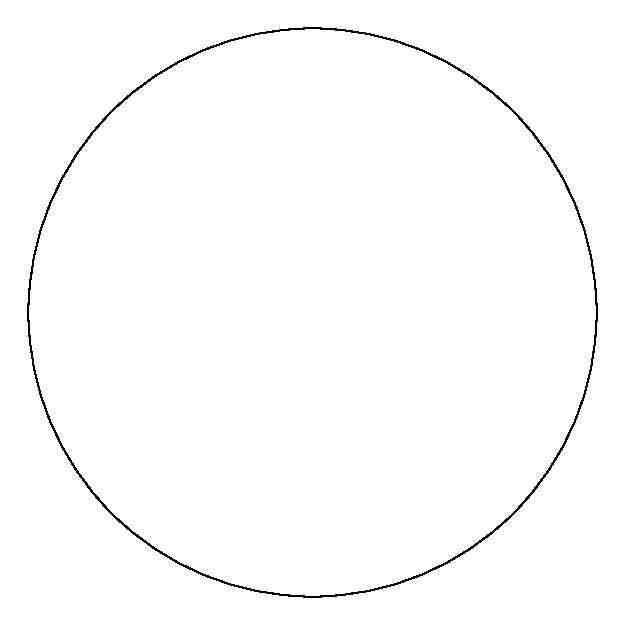
\includegraphics[height=4cm]{arc-length/pictures/09-01-circlea.pdf}%
%}%
%\only<handout:0| 3>{%
%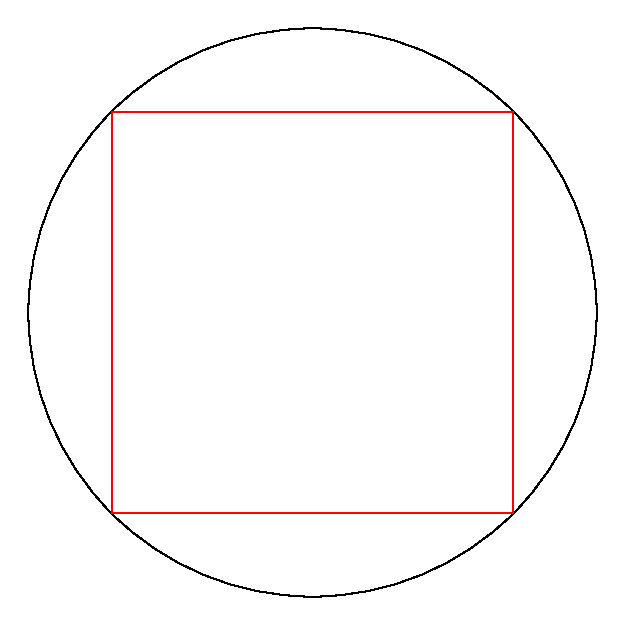
\includegraphics[height=4cm]{arc-length/pictures/09-01-circleb.pdf}%
%}%
%\only<handout:0| 4>{%
%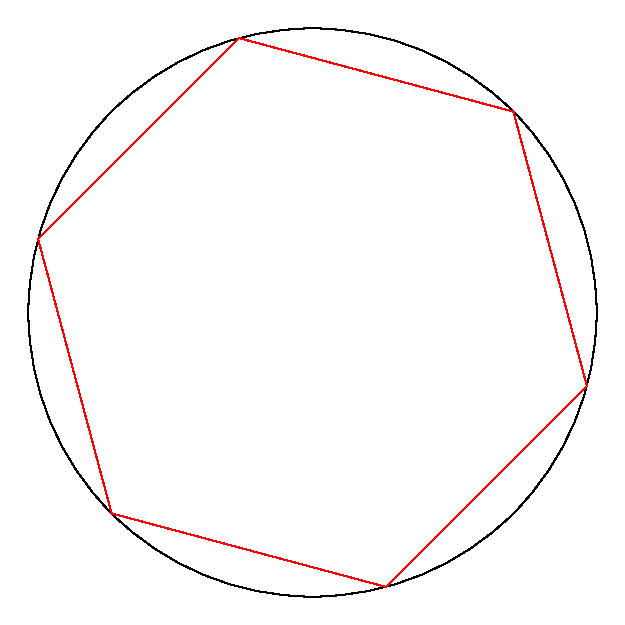
\includegraphics[height=4cm]{arc-length/pictures/09-01-circlec.pdf}%
%}%
%\only<handout:0| 5>{%
%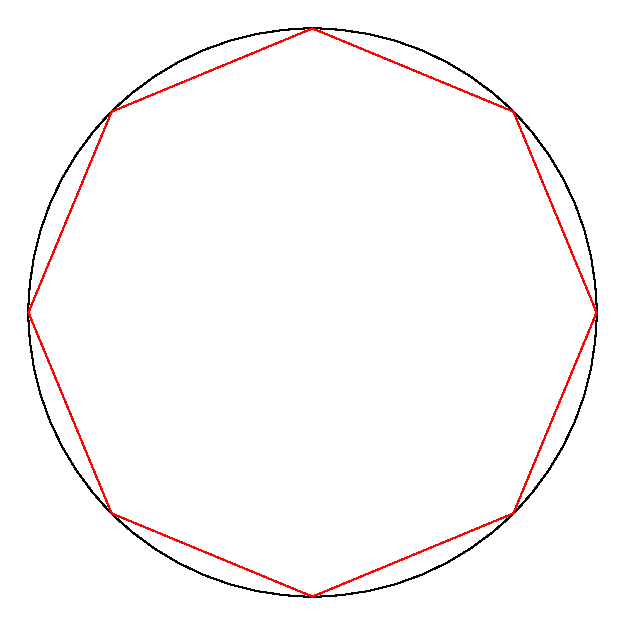
\includegraphics[height=4cm]{arc-length/pictures/09-01-circled.pdf}%
%}%
%\only<handout:0| 6>{%
%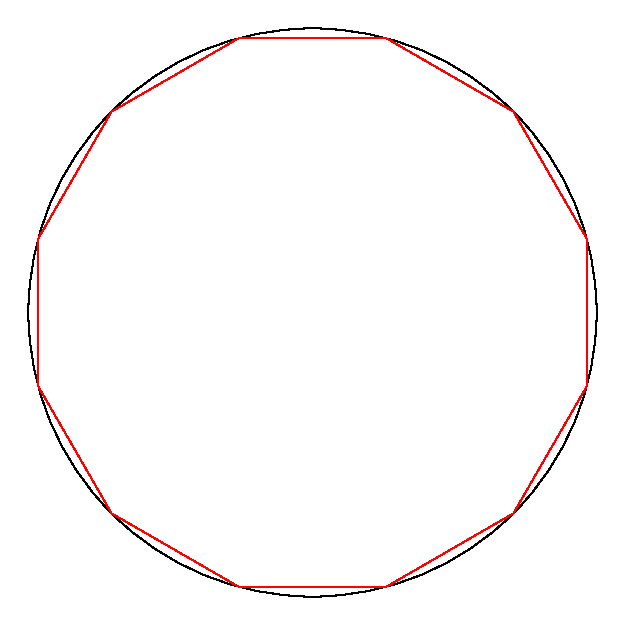
\includegraphics[height=4cm]{arc-length/pictures/09-01-circlee.pdf}%
%}%
%\only<handout:0| 7->{%
%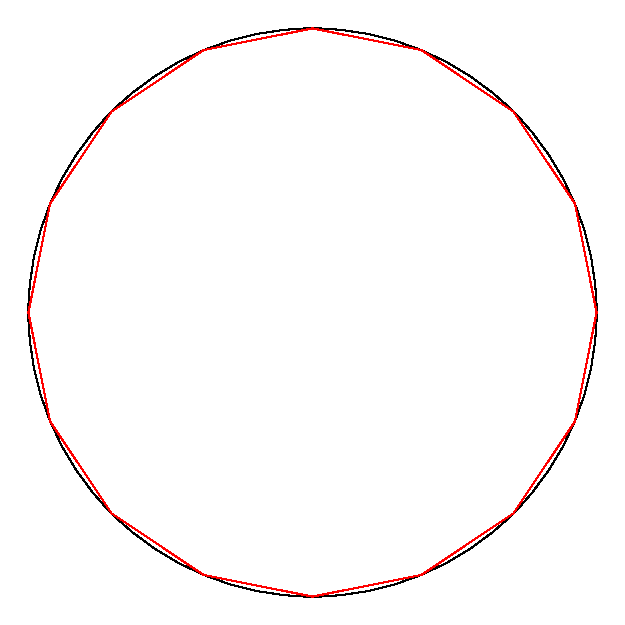
\includegraphics[height=4cm]{arc-length/pictures/09-01-circlef.pdf}%
%}%
%\end{center}
\begin{itemize}
\item  What do we mean by the length of a curve?
\item<2->  The length of a polygon is easy to compute: add up the length of the line segments that form the polygon.
\item<3->  If the curve is a circle, approximate it by a polygon.
\item<4->  Then take the limit as the number of segments of the polygon goes to $\infty$.
\end{itemize}
\end{frame}
% end module arc-length-intro
